%\documentclass{cumcmthesis}
\documentclass[withoutpreface,bwprint]{cumcmthesis} %去掉封面与编号页,电子版提交的时候使用。
\usepackage[superscript]{cite}
\usepackage{booktabs}
\usepackage{longtable}
\usepackage{float}
\usepackage{graphicx}
\usepackage{float}
\usepackage[framemethod=TikZ]{mdframed}
\usepackage{url}   % 网页链接
\usepackage{subcaption} % 子标题
\usepackage[linesnumbered,ruled,vlined]{algorithm2e} 
\usepackage{adjustbox}
\usepackage{algpseudocode}
\title{数学建模论文排版}
 
\begin{document}
\maketitle
\begin{abstract}

	这里写摘要,国赛论文摘要要求是一页最好,不要多也不要太少。

	%\keywords{ 科幻小说 \quad  摘要 \quad 三体  \quad  关键字 \quad 科学边界}
	\noindent{ \textbf{关键词:} Fisher精确检验\quad   多元线性回归\quad 系统聚类 \quad 灰色关联分析\quad}
\end{abstract}


\section{问题重述}
某电子产品的生产企业需要综合诸多考虑购置零部件、产品抽检、产品拆解、报废等问题,以确保产品质量的同时降低成本。

\textbf{问题一:}考虑到零配件供应商所述次品率不高于既定标称值,企业拟采用抽样检测方法以验收此批零配件。因为企业寻承担检测费用,企业希望应用数学模型得到最少抽检次数的抽样方案。

已知标称值为 10\%,结合以下两种不同情况,分别设计出具体的抽样检测方案:

1. 拒收条件:在95\%的置信水平下,如果检测结果表明零配件的次品率超出了标称值,那么这批零配件将被拒收。

2. 接收条件:在90\%的置信水平下,如果检测结果表明零配件的次品率未超过标称值,那么这批零配件将被接收。

\textbf{问题二:}在已知零配件及成品次品率情况下,在电子产品生产的零配件检测、装配、成品检测、不合格品拆解的各个阶段为企业作出最优决策。
并且结合判断依据及相应的指标对表1中企业在生产中遇到的情况作出相应的最优决策方案。

\textbf{问题三:}在零配件、半成品和成品的次品率已知情况下,重复问题2的生产决策方案以适配有m道工序、
n个零配件的问题。并且应用此方法针对表2中情况给出判断依据和指标得到最优的决策方案。

\textbf{问题四:}在零配件、半成品和成品的次品率均由抽样检测获得的情况下,重新考虑问题2、3的生产决策方案。
\section{问题分析}
\subsection{问题一的分析}
我们需要根据题目中给出的两种不同的情况,分别设计抽样检测方案。考虑单次检验为次品严格服从经典二项分布
,拟采用异常检测的经典取样方法:序贯概率比检测$SPRT$来动态地作出抽样决策。

\subsection{问题二的分析}
由于已知各零配件以及成品的次品率,依据排列组合我们能够得知在生产成品时零配件优劣的组合情况以及对应的概率分布。
又由于可能出现两个好的零部件组成一个坏的成品,综合成本考量我们是否需要考虑对成品进行拆解。
我们预先设置对零配件、成品的抽样检测参数(即:抽检/不抽检),通过多次模拟迭代实验得到最优的检测方案,以此来减少检测次数。
\subsection{问题三的分析}

\section{基本假设与符号说明}
\subsection{基本假设}
$\bullet$ 假设理论物理跟泵不存在;

$\bullet$ 假设数据中未填写的数据项为 0

$\bullet$ 假设所提供的数据准确无误;

$\bullet$ 不考虑因检验手段等原因对数据值的影响。

\subsection{符号说明}
\begin{table}[H]
	\centering
	\setlength{\tabcolsep}{20mm}%调整长度
	\begin{tabular}{cc}
		\toprule[1.5pt]
		\textbf{符号} & \textbf{含义}   \\  %textbf可以给文字加粗
		\midrule[1pt]
		$N$         & 每批供应商提供的零配件总量 \\
		$D_{i}$     & 第$i$次抽检的零配件数量 \\
		$\mu$       & 次品率           \\
		$A$         & 拒真的决策边界       \\
		$B$         & 纳伪的决策边界       \\
		$LR$        & 似然比           \\
		\bottomrule[1.5pt]
	\end{tabular}
\end{table}

\section{问题一模型的建立与求解}
针对每批零配件,假定总量为$N$,我们考虑采用异常检测的经典取样方法:序贯概率比检测$SPRT$作为抽检方案。在此之前
我们考虑每次取样的样本量为$D_i$,令单个零件次品与否的布尔值为$x$,考虑其单次试验成功(为次品)概率的期望为$\mu$,则其显然
服从经典的二项分布表示:
\begin{equation}
	\textit{Bern}(x|\mu) = \mu^x (1 - \mu)^{1-x}
\end{equation}
接下来考虑其在样本集上的对数似然函数,针对第$i$次取样$D_i$,对其中的每个样本取到观测$x_1,x_2...x_n$,根据题目要求
样本集中零配件的次品产生事件可认定为相互独立的。则其似然函数可写为:
\begin{equation}
	\mathbf{P}(D_i|\mu) = \prod_{n=1}^{N} p(x_n|\mu) = \prod_{n=1}^{N} \mu^{x_n} (1 - \mu)^{1-x_n}
\end{equation}
为便于后续处理,我们取其对数似然:
\begin{equation}
	\begin{split}
		&\ln\mathbf{P}(D|\mu) = \ln \prod_{n=1}^{N} \mu^{x_n} (1 - \mu)^{1-x_n}
		= \ln \mu \sum_{n=1}^{N} x_n + \ln(1 - \mu) \sum_{n=1}^{N} 1 - x_n \\
		&=  \ln \mu \sum_{n=1}^{N} x_n + \ln(1 - \mu) (N - \sum_{n=1}^{N} x_n)
		= \sum_{n=1}^{N} x_n \ln \mu + (1 - x_n) \ln(1 - \mu)
	\end{split}
\end{equation}
接下来我们依据题干给定零假设和备择假设:
\begin{equation}
	\begin{cases}
		H_0: \mu > 0.1 \\
		H_1: \mu \le 0.1
	\end{cases}
\end{equation}
题干中的两种情况意味着拒真和纳伪的显著性水平$\alpha$和$\beta$分别为0.05和0.1。在\textit{SPRT}语境下,考虑决策边界:
$$ A = \ln \frac{\beta}{1 - \alpha} \ \ \ \  B = \ln \frac{1 - \beta}{\alpha}$$
于是,针对每次采样$D_i$,我们需要求出在零假设和备择假设下的似然比$LR$:
\begin{equation}
	LR= \frac{\sum_{n=1}^{N} x_n \ln \mu_0 + (1 - x_n) \ln(1 - \mu_0)}{\sum_{n=1}^{N} x_n \ln \mu_1 + (1 - x_n) \ln(1 - \mu_1)}
\end{equation}
需要注意的是,在原生的$SPRT$场景中,$H_0$和$H_1$一般被认定为较为复杂的参数估计$\theta_0$和$\theta_1$,这取决于它们事先假定样本服从一个较为严谨且高度可表达的
概率分布。然而基于问题一,在没有明确历史数据和概率分布的先验情况下,我们只能将其建模为一般二项分布,
为了遵循$SPRT$的使用场景,我们将二项分布参数建模为$\mu_0=0.1+\Delta \mu_0$ , $\mu_1=0.1-\Delta \mu_1$。通过轻微扰动量来拟合样本的分布与所报标称值
的差异,扰动量的设置取决于样本量的大小,这点我们将在后续给出实验和说明。

尽管在许多场景中单样本取样策略以及被证明取得了很好的效果,但考虑到题干背景,我们依然选择样本集作为采样标准。遵循$SPRT$方法,给定总零配件量$N$,初次取样
$D_i$应为按照标称值所取的总样本配比,我们取$D_1=0.01N$,而后计算出当前样本下的对数似然比$LR_1$。序贯检验比方法遵循以下停止法则:
\begin{equation}
	\gamma = \inf \left\{ n | n \geq 1, LR_n \in (A, B) \right\}
\end{equation}
具体来说,若$LR_1 \le A$,接受$H_0$假设;若$LR_1 \ge B$,接受$H_1$假设,否则继续采样。初次采样的样本量为$D_1=0.01N$,假定每次
采样的次品数为$n_i$,则此后每次采样量依据以下法则确定:
\begin{equation}
	D_{i+1}=D_i-n_i
\end{equation}
检验的完整流程可以作出如下表表示:

\begin{adjustbox}{width=16cm,height=6.5cm}
	\centering
	\begin{algorithm}[H]
		\SetAlgoLined
		\KwIn{总零配件数量 $N$,显著性水平 $\alpha$,第二类错误概率 $\beta$,扰动量 $\Delta \mu_0,\Delta \mu_1$}
		\KwOut{接受的假设 ($H_0$ 或 $H_1$)}
		计算决策边界 $A \gets \ln \frac{\beta}{1 - \alpha}$, $B \gets \ln \frac{1 - \beta}{\alpha}$\;
		设置 $\mu_0 \gets 0.1 + \Delta \mu_0$, $\mu_1 \gets 0.1 - \Delta \mu_1$\;
		初始样本量 $D_1 \gets 0.01N$n\;
		$i \gets 1$\;
		\While{TRUE}{
			取样 $D_i$ 个零配件,记录次品数量 $n_i$\;
			计算 $LR_i$:
			\[ LR_i = \frac{\sum_{n=1}^{D_i} x_n \ln \mu_0 + (1 - x_n) \ln(1 - \mu_0)}{\sum_{n=1}^{D_i} x_n \ln \mu_1 + (1 - x_n) \ln(1 - \mu_1)} \]
			\If{$LR_i \le A$}{
				接受零假设 $H_0$; \textbf{break}
			}
			\ElseIf{$LR_i \ge B$}{
				接受备择假设 $H_1$; \textbf{break}
			}
			\Else{
				$i \gets i+1$; $D_{i+1} \gets D_i - n_i$ \ \ 继续执行采样策略
			}
		}
		\Return 接受的假设 ($H_0$ 或 $H_1$)
		\label{alg:sprt}
		\caption{序贯概率比检验 (SPRT) 流程}
	\end{algorithm}
\end{adjustbox}

接下来我们考虑之前我们搁置的$\Delta \mu$的选取,这是该方案唯一的松弛参数;我们希望把它建模成一个函数而非定量。
这是由于我们面临一个相当大的搜索空间,它主要取决于两个因素:(1)总零配件数量$N$,由于该变量我们是不可控且无
先验的,所以我们暂且假定它的范围波动为$[1000,1000000]$;(2)真实标称值(Ground Truth) 我们也预先假定它的范围
波动为$[5\%,15\%]$。$\Delta \mu$的确定直接意味着SPRT策略的固定,面对庞大的搜索空间这样做显然是欠鲁棒的,因此寻找一种
对$\Delta \mu$的拟合$\Delta \mu = f(N,\theta)$是迫在眉睫的。其中N作为零配件总数是我们面临实际场景时的唯一自变量。$\theta$是拟合函数
的待优化参数。目标函数应该考虑到:(1)优化项:即尽可能减少取样量$D$;(2)惩罚项:即不出现误判的情况。于是它可以设计为:
\begin{equation}
	\Delta \mu = f(N,\theta) \ \ \ \ \ \ s.t. \ \underset{\theta}{\operatorname{argmax}} \ (\frac{1}{D} \times \mathbf{1}_H)
\end{equation}
这里的$\mathbf{1}_H$是对假设H的指示函数,用以表示最终选取的假设是否为真。
我们使用多层感知机(MLP)去拟合函数$f(N,\theta)$,自定虚拟数据集的范围遵循前文中给出的零件数量$N$和真实标称值的波动范围。
在1000个epoch中,我们选取测试集中精度最高的MLP模型作为评估基线以衡量SPRT的表现情况。最终结果如图所示:
\section{问题二的模型建立与求解}
首先,我们可以将电子产品加工过程分为三个阶段,即:零配件、成品、市场。每当生产过程从一个阶段进入到另一个阶段均需要决策是否需要
进行抽检,将此过程抽象为图\ref{fig:pro2}。
\begin{figure}[H]
	\centering
	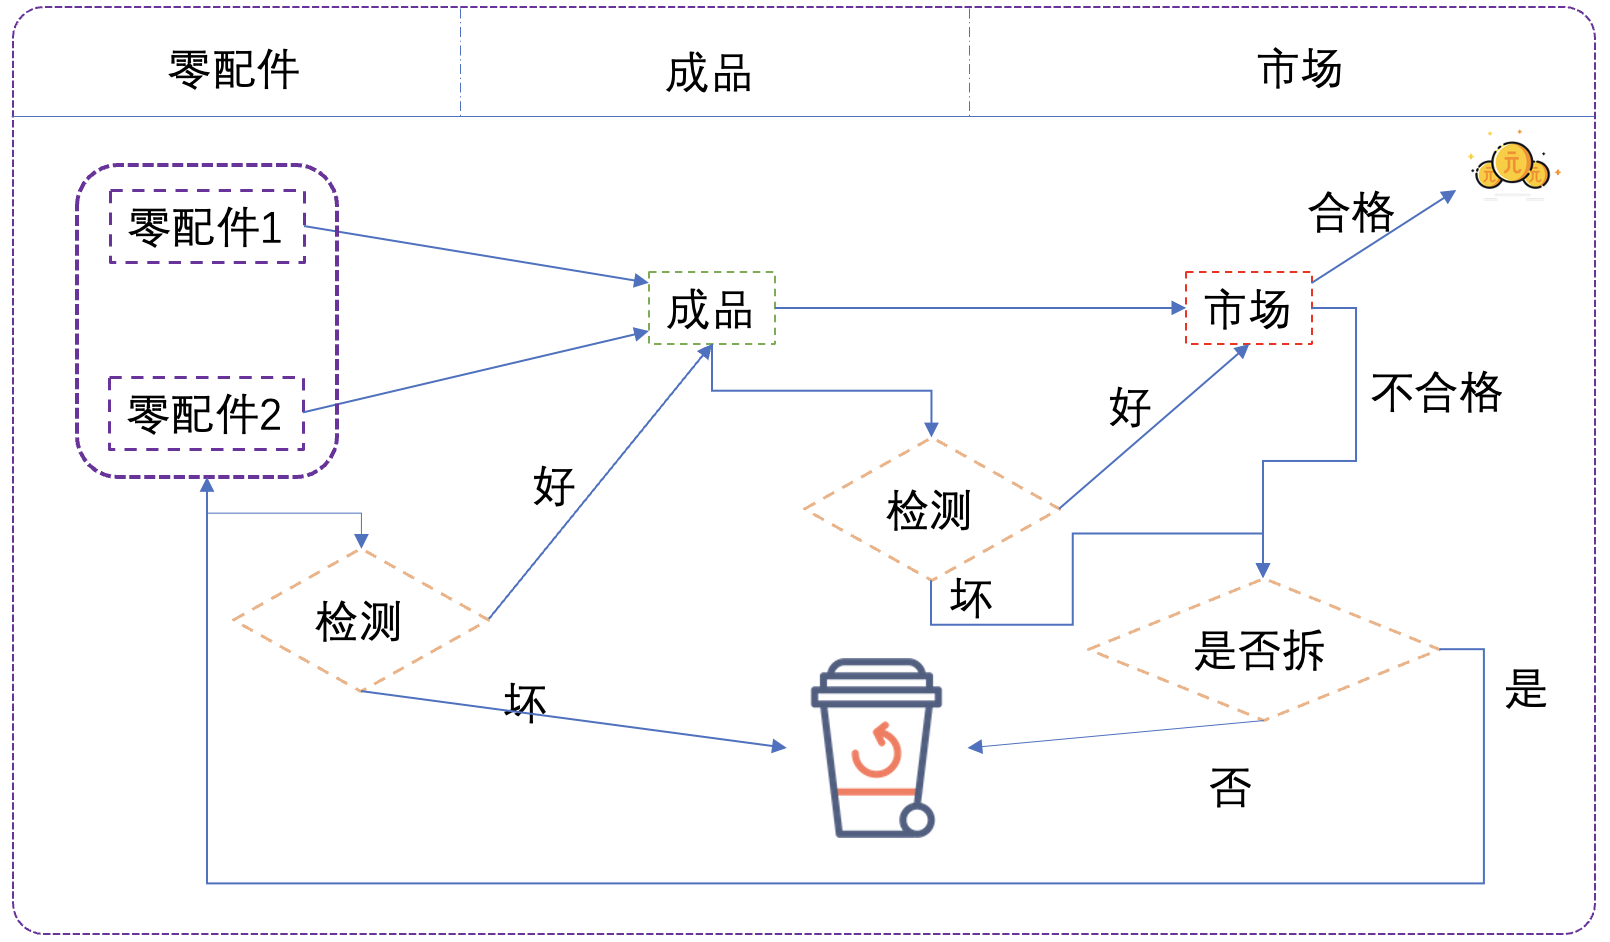
\includegraphics[width=0.6\textwidth]{Fig/pro2.png}      %获得的图片花括号中的名称为figure文件夹中重命名后的图片
	\caption{电子器件生产的流程图}
	\label{fig:pro2}
\end{figure}
\subsection{模型的建立}
在生产过程中我们设置一个列向量$C=(c_{1},c_{2},c_{3},c_{4})^{T}$,其中的元素$c_i$分别表示
零配件1、零配件2、成品是否抽检及检测到不合格的成品是否拆解($c_{i}$的值为0时表示为不抽检/不拆解(丢弃),值为1时表示检测/拆解)。
我们的目标是通过合理的决策方案使得纯利润的期望值最最大。

因为零部件及成品的次品率已知,在每批零配件数目$N$足够大的情况下,我们可以通过对正次品进行排列组合,算出成品中的正次品零部件各种组合的概率。
在这里假设每批投入零部件1和零部件2的数目分别为$N_{1}$和$N_{2}$(这里的$N$足够大),其中$\mu_{1}$和$\mu_{2}$分别为零部件1、2的次品率,
则近似可以认为供应商提供的零部件1、2的次品数目为$N_{1}\cdot\mu_{1}$和$N_{2}\cdot\mu_{2}$。先考虑对零部件不进行检测直接拼装为成品的
情况,可以得出存在零部件次品的成品数目$k$的值域为$[\max \{N_{1}\cdot\mu_{1},N_{2}\cdot\mu_{2} \},N_{1}\cdot\mu_{1}+N_{2}\cdot\mu_{2}]$。
令$k$个成品中存在$i$和$j$个零配件1、2的次品个数。可以得到成品中有$i$个零配件1和$j$个零配件2的概率为$P_{i,j}$,计算公式如下:
\begin{equation}
	P_{i,j}=C_{N_{1}\cdot\mu_{1}}^{i}C_{N_{2}\cdot\mu_{2}}^{j}\mu_{1}^{i}\mu_{2}^{j}(1-\mu_{1})^{k-i}(1-\mu_{2})^{k-j}
	\label{eq:1}
\end{equation}
则$i$和$j$应当满足$i+j\ge k,i\le k,j\le k$,经过计算得到i和j的取值范围为$[k-j,k]$和$[\frac{k}{2},k]$。
我们假设$P_{k}$为存在次品零部件的成品数目为$k$的概率,计算公式如下:
\begin{equation}
	P_{k}=\sum_{i=k-j}^{k}\sum_{j=\frac{k}{2}}^{k}C_{N_{1}\cdot\mu_{1}}^{i}C_{N_{2}\cdot\mu_{2}}^{j}\mu_{1}^{i}\mu_{2}^{j}(1-\mu_{1})^{k-i}(1-\mu_{2})^{k-j}
	\label{eq:2}
\end{equation}

为了更直观的得到不同决策向量对电子产品生产的收益的影响,我们将图\ref{fig:pro2}中的单次生产流程抽象为一个生产轮次。在每个轮次中我们假设每轮
接受供应商提供的配件数目为固定的$N_{1}$、$N_{2}$,经过上一轮被检测为次品的零部件全部被舍弃,被拆解的成品中的零配件投入下一轮次的零配件池进入生产。
在每轮次生产中我们需要确定不同决策向量以保证电子产品生产的收益,于是我们拟定$t$个生产轮次为一个生产周期,每个生产周期中决策向量$C^{*}=(c_{1},c_{2},\dots,c_{4t})$
为$t$个生产轮次中决策列向量$C$的叠加,如图\ref{fig:pro2-2}。
\begin{figure}[H]
	\centering
	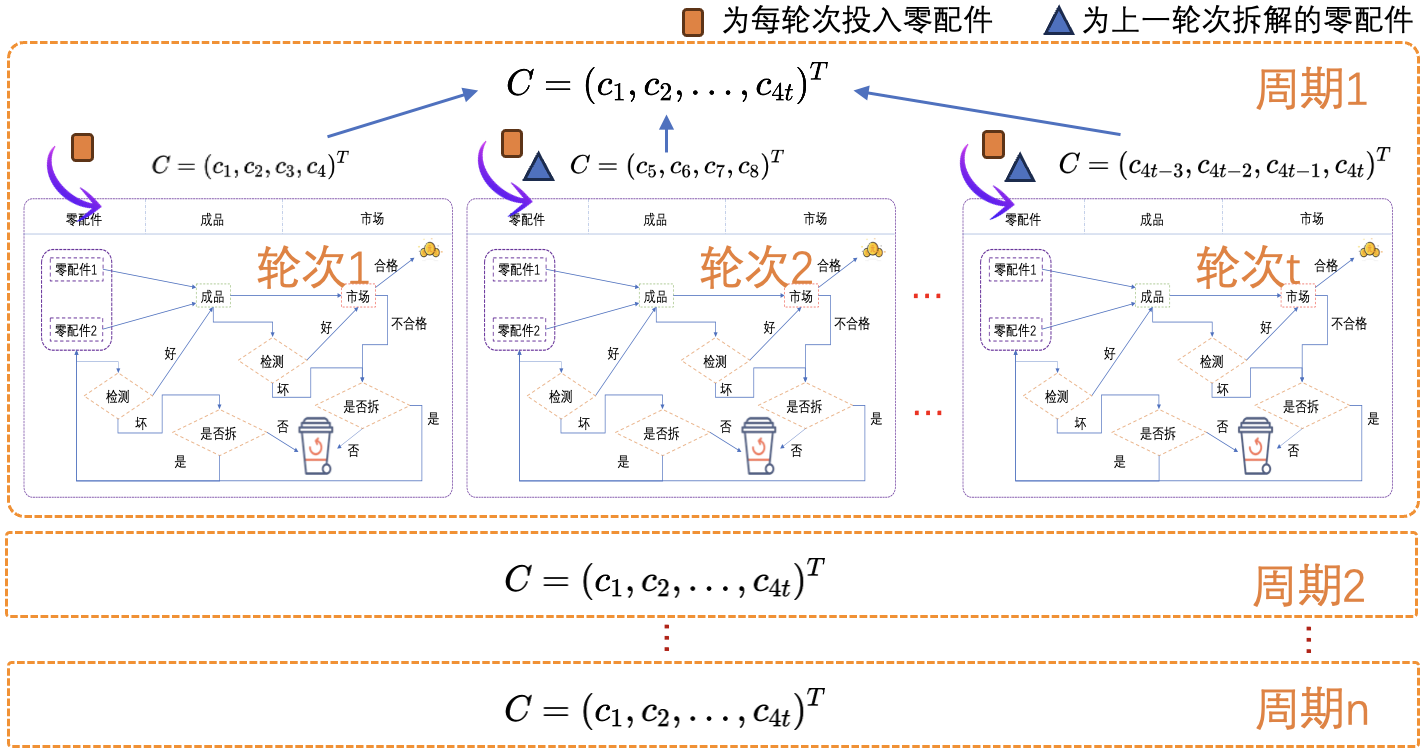
\includegraphics[width=0.8\textwidth]{Fig/pro2-2.png}      %获得的图片花括号中的名称为figure文件夹中重命名后的图片
	\caption{产品迭代周期图}
	\label{fig:pro2-2}
\end{figure}

\subsection{模型的求解}

\end{document}
